% Application of lpreba package

%%%% Preamble %%%%

\documentclass[a4paper, 12pt]{scrartcl}

% Packages

% General
\usepackage{lmodern}
\usepackage[hidelinks]{hyperref}

% Spacing
\usepackage{geometry}
	\geometry{a4paper, top=2cm, left=2cm, right=2cm, bottom=2cm, footskip=1.25cm}
\usepackage[onehalfspacing]{setspace}
\setcapindent{0pt}

% Plotting
\usepackage{graphicx}
	\graphicspath{{figures/}}
\usepackage{subcaption}
\usepackage[nomarkers, figuresonly, nofiglist]{endfloat}
	\renewcommand{\efloatseparator}{\vfill}

% Bibliography
\usepackage[backend=biber, style=authoryear, maxcitenames=2]{biblatex}
\addbibresource{application.bib}
\renewbibmacro{in:}{}
\renewbibmacro{volume+number+eid}{
	\printfield{volume}
	\setunit{\addnbthinspace}
	\printfield{number}
	\setunit{\addcomma\space}
	\printfield{eid}}
\DeclareFieldFormat[article]{number}{\mkbibparens{#1}}
\DeclareFieldFormat{url}{\url{#1}}
\renewcommand{\nameyeardelim}{\addcomma\space}

%%%% Document %%%%

\begin{document}

\begin{center}
	\textsf{\textbf{\Large Application of \texttt{lpreba} package}}
\end{center}
\noindent
To showcase the practical use of the \texttt{lpreba} package,
we consider the nonparametric estimation of treatment effects in the regression discontinuity design (RDD).
RDD is a popular quasi-experimental research design to identify a causal effect
as a jump of an outcome variable at a known threshold of a so-called assignment variable.
This threshold constitutes a boundary.
When measuring the size of the discontinuity, i.e.\ the causal effect in a valid RDD,
boundary effects may severely bias the estimate and inference.
RDD was first applied by \textcite{Thistlethwaite_1960}.
\textcite{Hahn_2001} were the first to suggest local linear regression to estimate the conditional expectation function
at the threshold to avoid boundary bias.
Also see \textcite{Porter_2003}.

In a widely-cited study, \textcite{Lee_2008} applied RDD to analyze the causal effect of party incumbency
on reelection probabilities in U.S. House elections.
Figure~\ref{fig:application_overview} shows the Democrats' probability of winning a seat in the U.S. House of Representatives
in the next election against the Democratic vote share minus the vote share of the strongest opponent
(almost always the Republicans).
Each data point is an average of the indicator variable for winning election $t+1$ for each interval, which is 0.005 wide.
To the left of the zero-threshold the Democratic nominee lost election $t$;
to the right, the Democratic party won.
We can see a smooth relationship between the two variables (higher reelection probability for a higher vote share),
except for the threshold at zero which decides about victory or defeat.
\textcite{Lee_2008} interprets the large discontinuity as the true electoral incumbency advantage
as he argues that due to the inherent uncertainty in the exact vote share,
winning a close election is ``as good as random''.
Then, districts where the Democrats just barely lost constitute a valid counterfactual for districts
where the Democrats just barely won and became incumbent (receiving treatment).

\begin{figure}
	\centering
	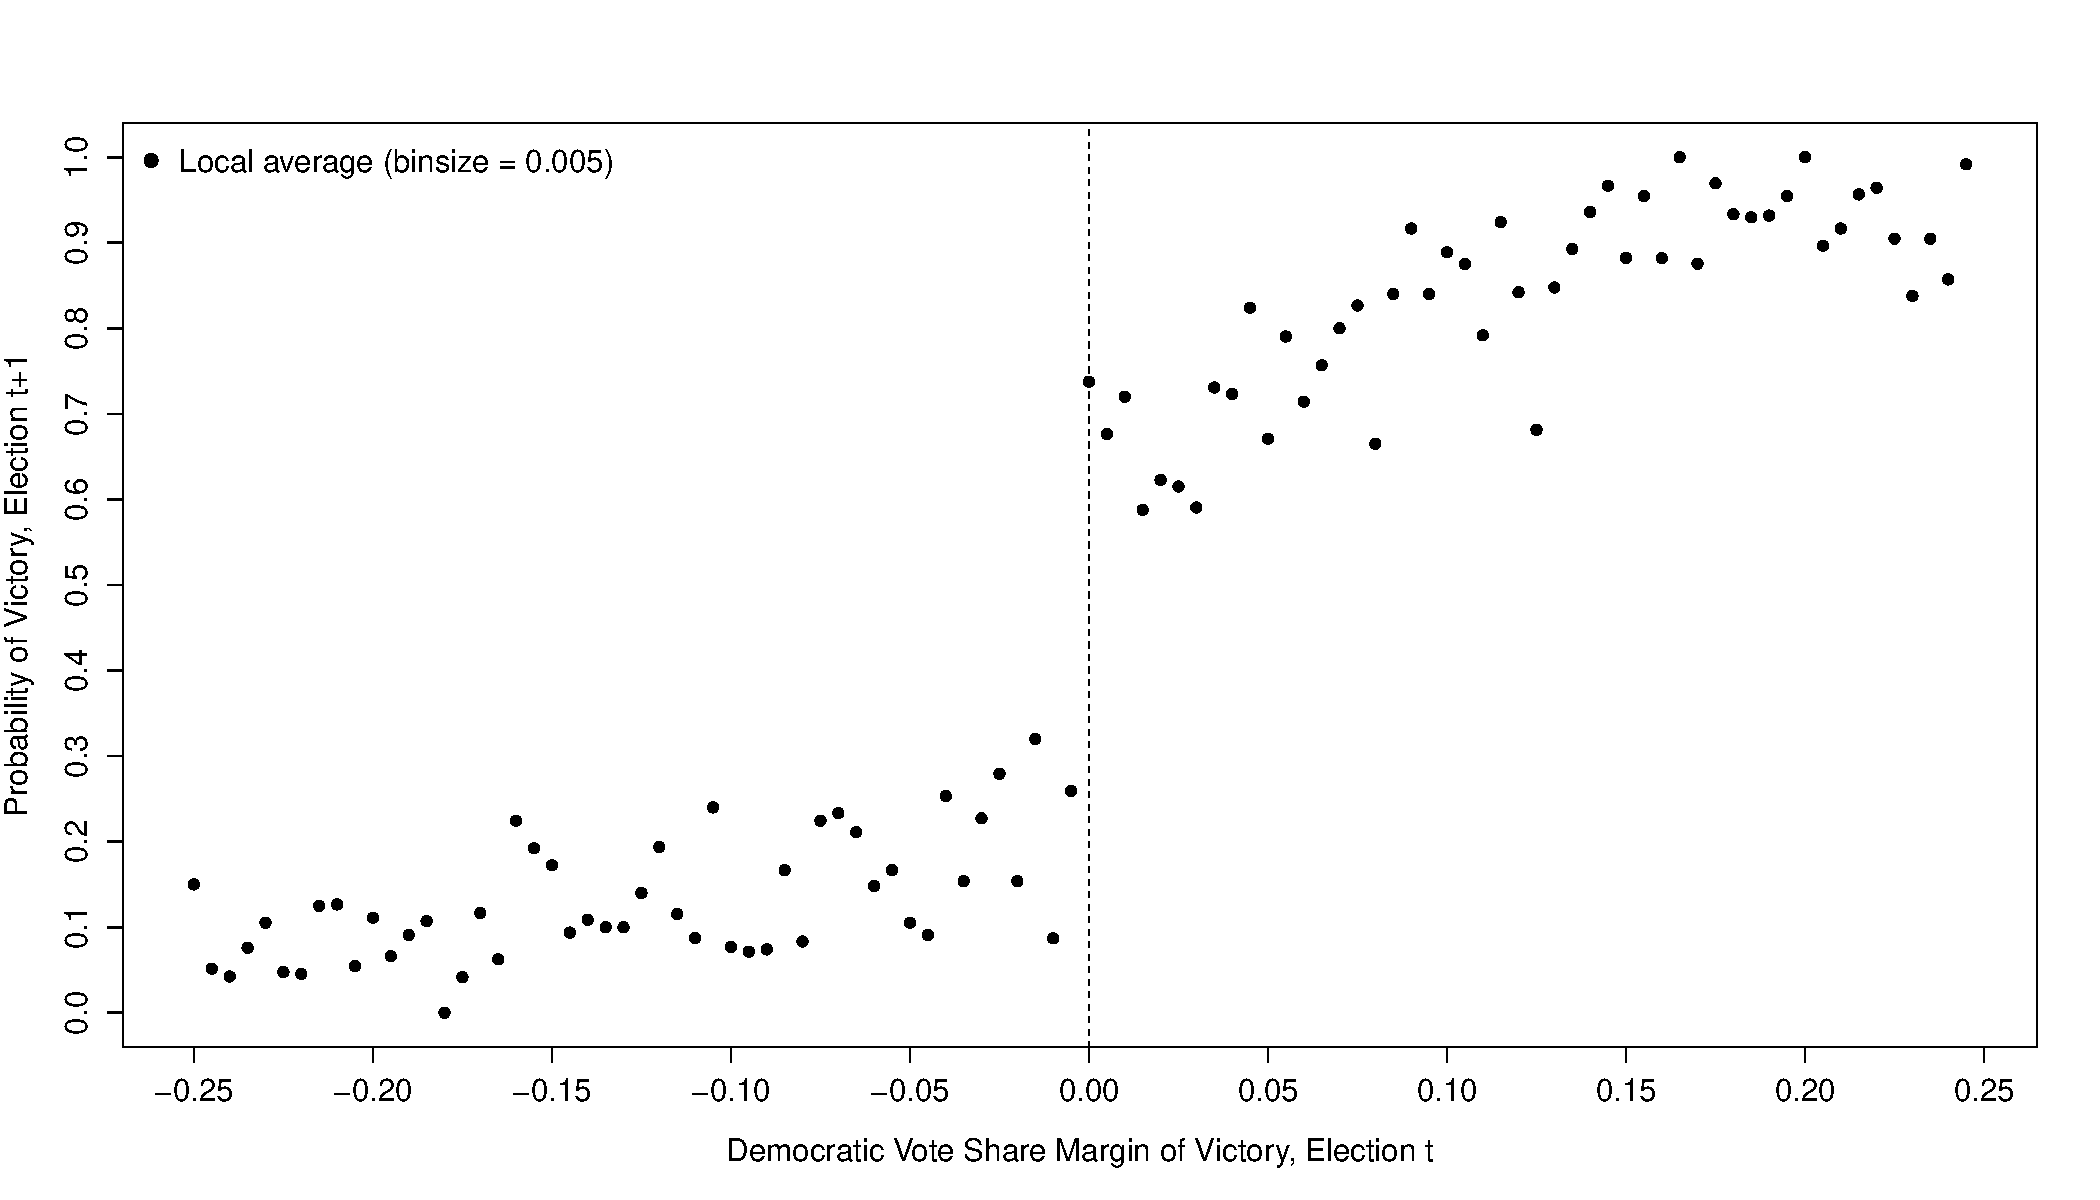
\includegraphics[trim=0 15 20 50, clip, width=\textwidth]{application_figure_01.pdf}
	\caption{Democrats' probability of victory in election $t+1$, by margin of victory in election $t$.
			 Local averages are given by the filled circles.}
	\label{fig:application_overview}
\end{figure}

The task is now to estimate the size of the discontinuity.
Figure~\ref{fig:application_fits} displays the fit of the Nadaraya-Watson, the local linear
and the boundary-adjusted Nadaraya-Watson estimator for each side of the threshold.
To select the bandwidths (we allow the degree of smoothing to differ for each side)
we use leave-one-out cross-validation (LOOCV).
The solution has to be obtained numerically, which can cause problems.
The CV error function can have multiple local minima (Figures~\ref{fig:application_left_nw}, \ref{fig:application_right_ll}),
and the solution can be unbounded (Figure~\ref{fig:application_left_ll}).
From the Figures~\ref{fig:application_left} and \ref{fig:application_right} we see that the cross-validated bandwidths
are larger for the left side and for the local linear estimator.

\begin{figure}
	\centering
	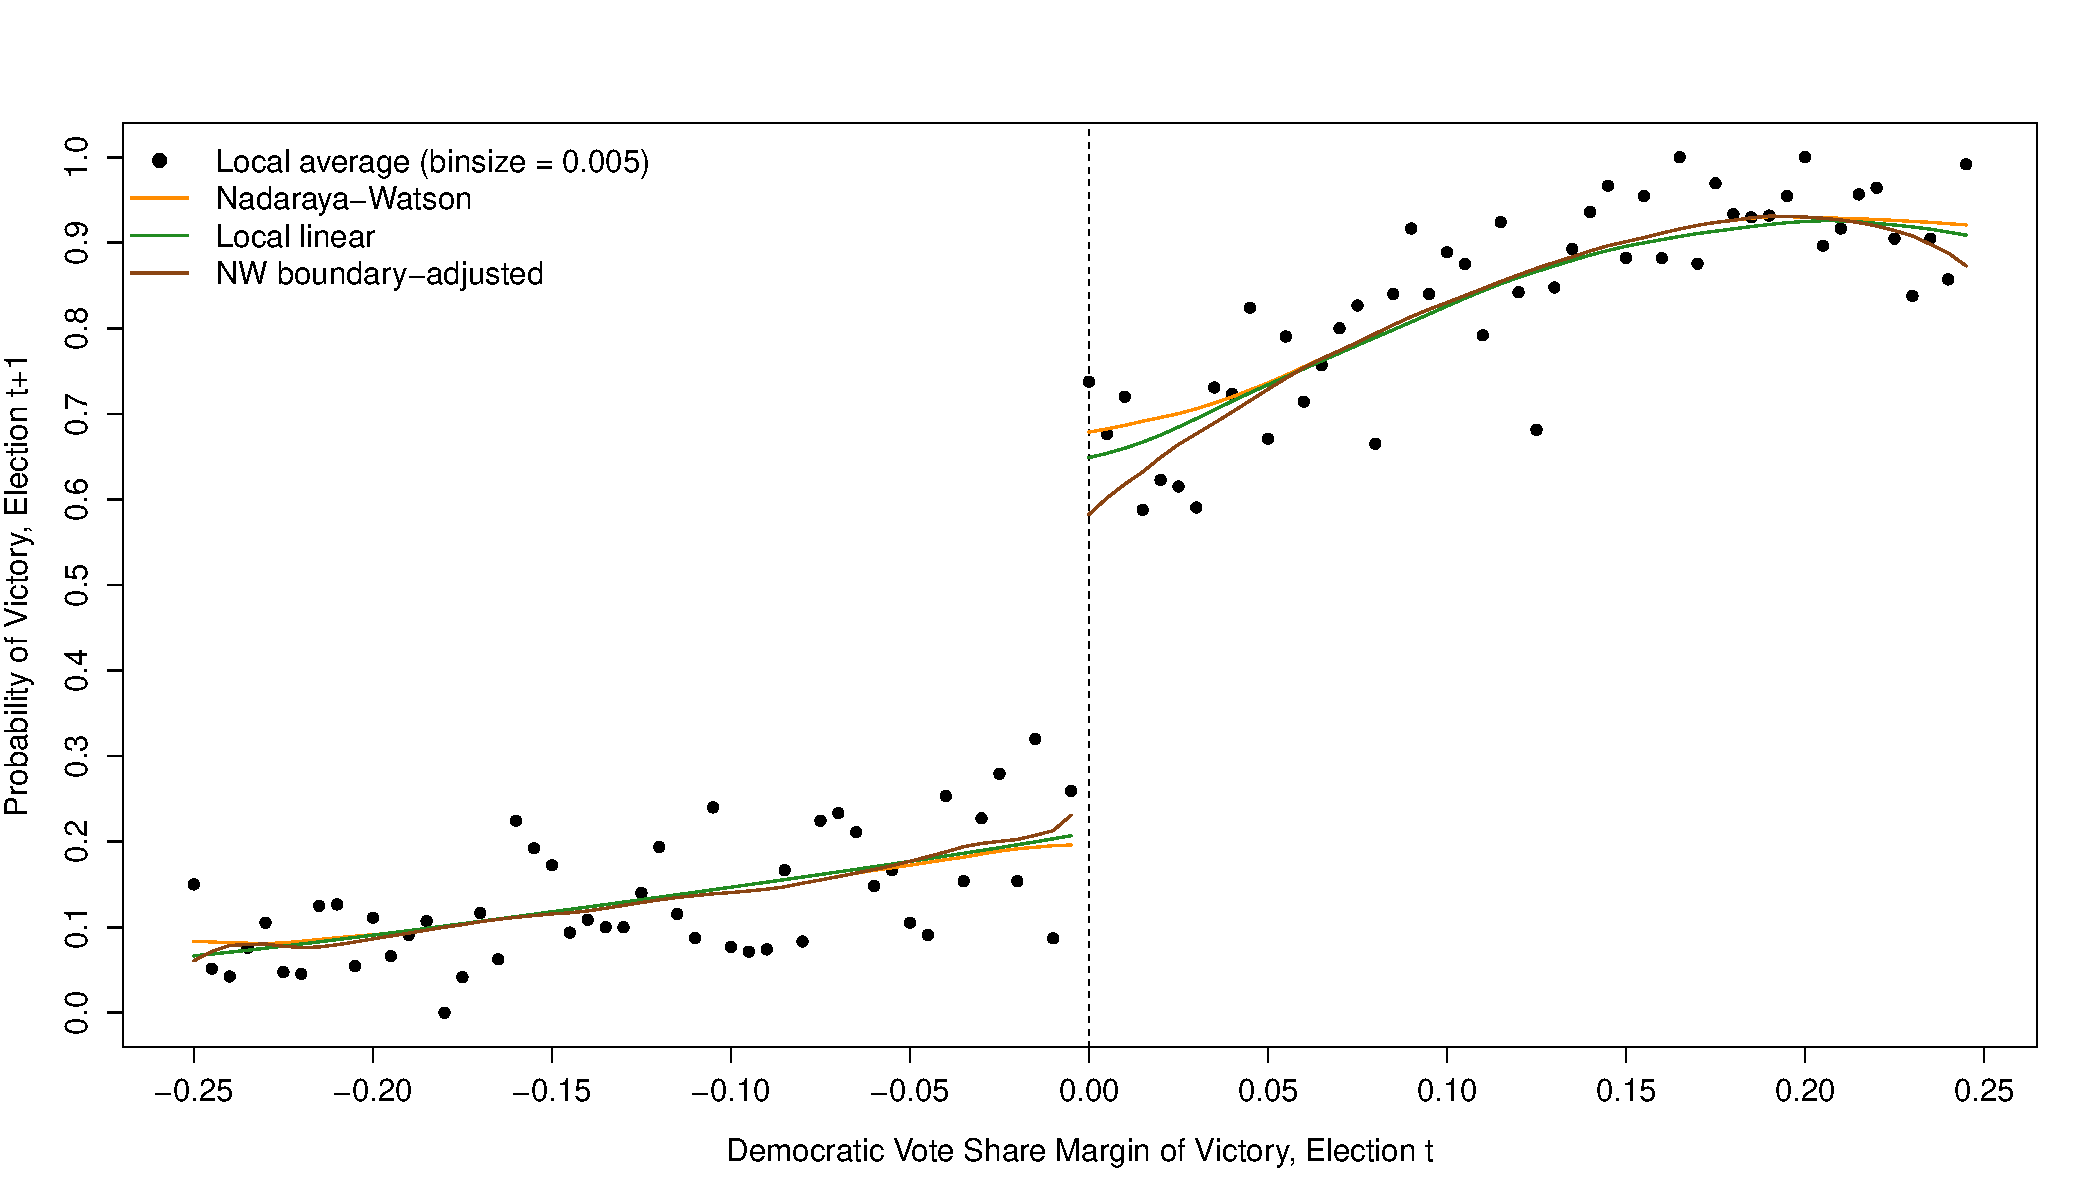
\includegraphics[trim=0 15 20 50, clip, width=\textwidth]{application_figure_02.pdf}
	\caption{Democrats' probability of victory in election $t+1$, by margin of victory in election $t$.
			 Estimates of Nadaraya-Watson, local linear regression and adjusted Nadaraya-Watson with cross-validated bandwidths.}
	\label{fig:application_fits}
\end{figure}

\begin{figure}
	\centering
	\begin{subfigure}{\textwidth}
		\centering
		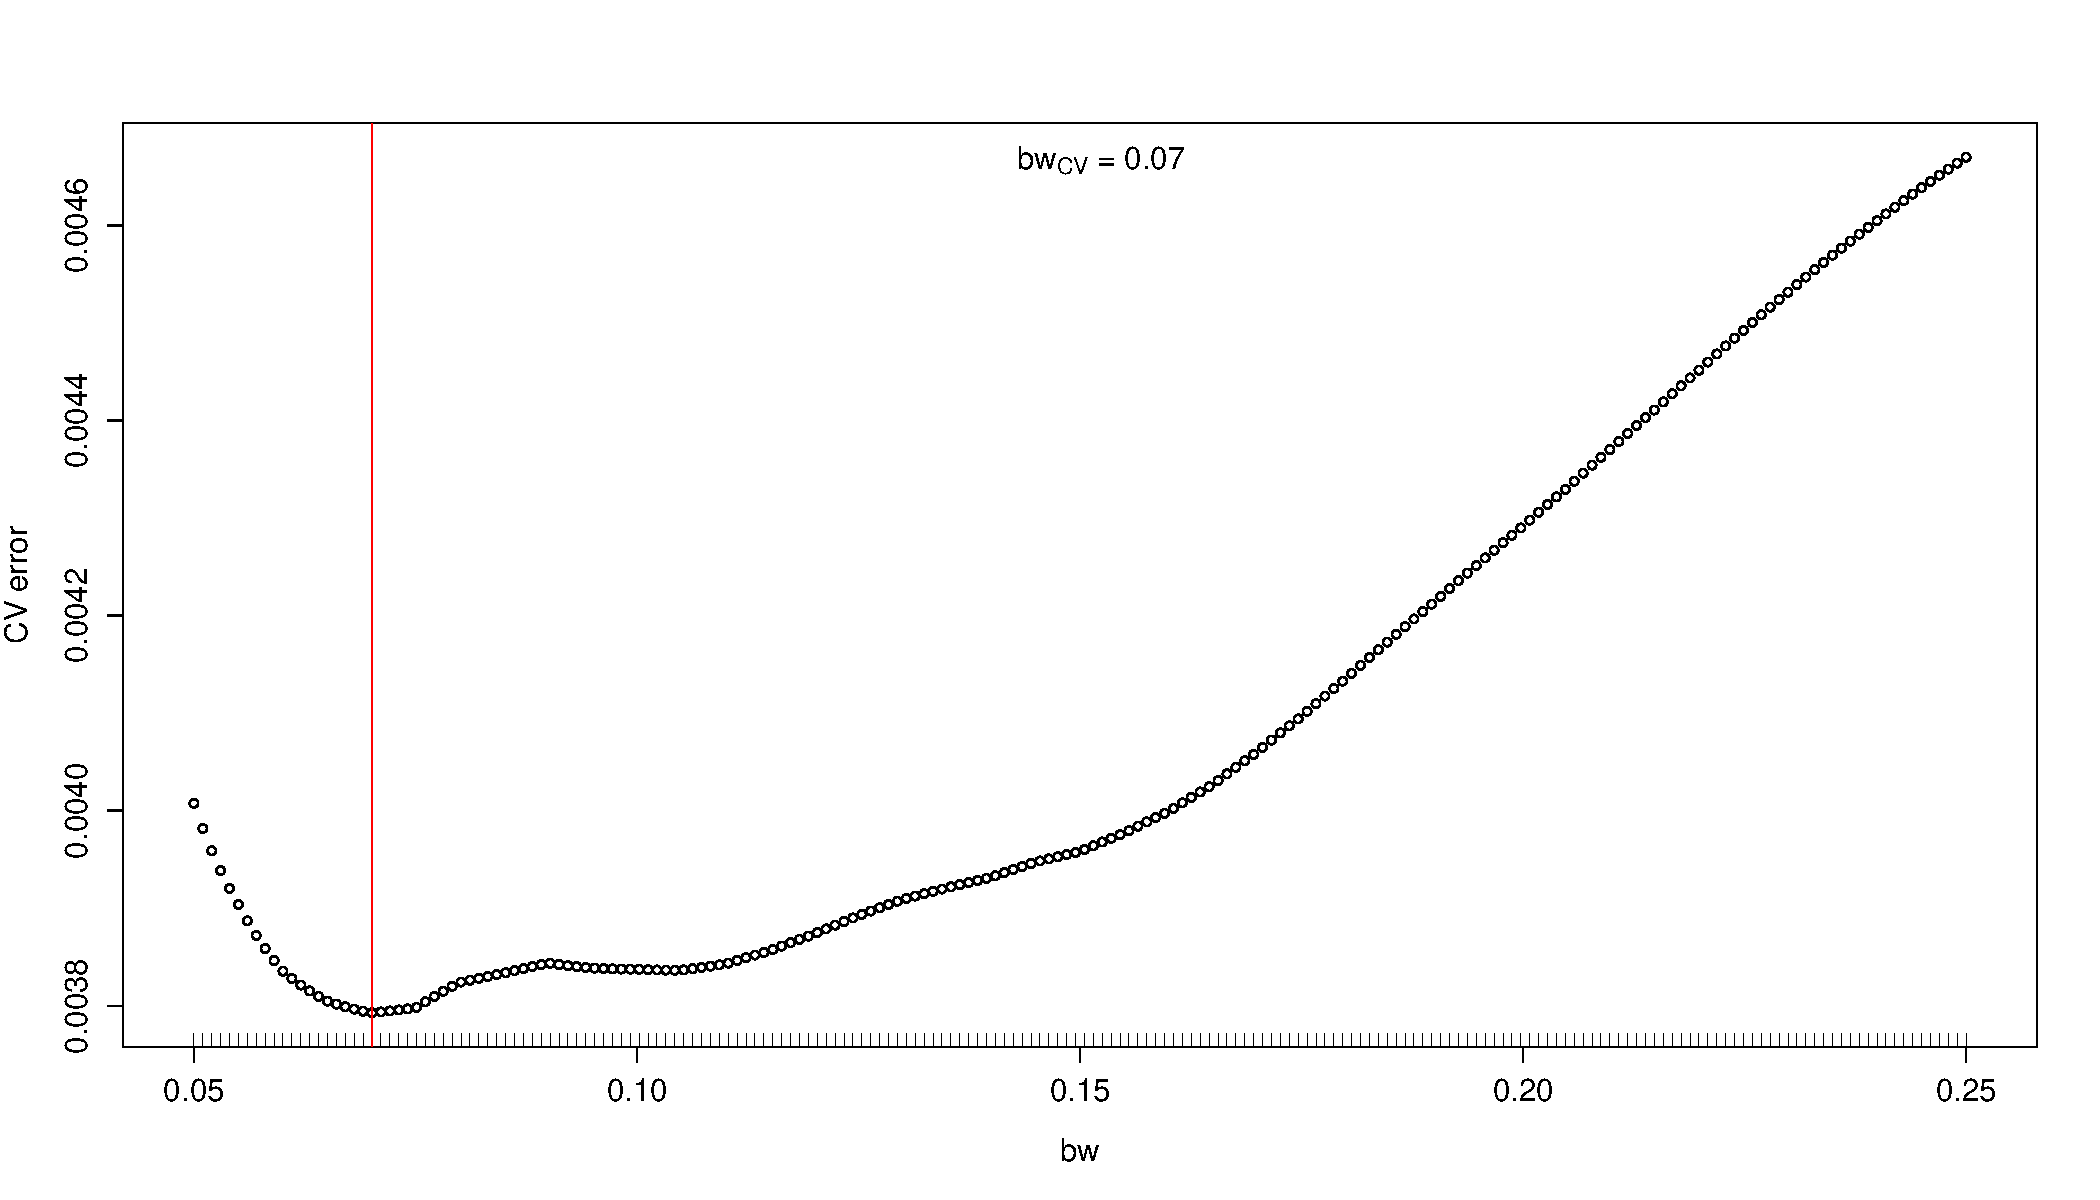
\includegraphics[trim=0 0 20 45, clip, width=\textwidth]{application_figure_03a.pdf}
		\caption{Nadaraya-Watson estimator}
		\label{fig:application_left_nw}
	\end{subfigure}

	\begin{subfigure}{\textwidth}
		\centering
		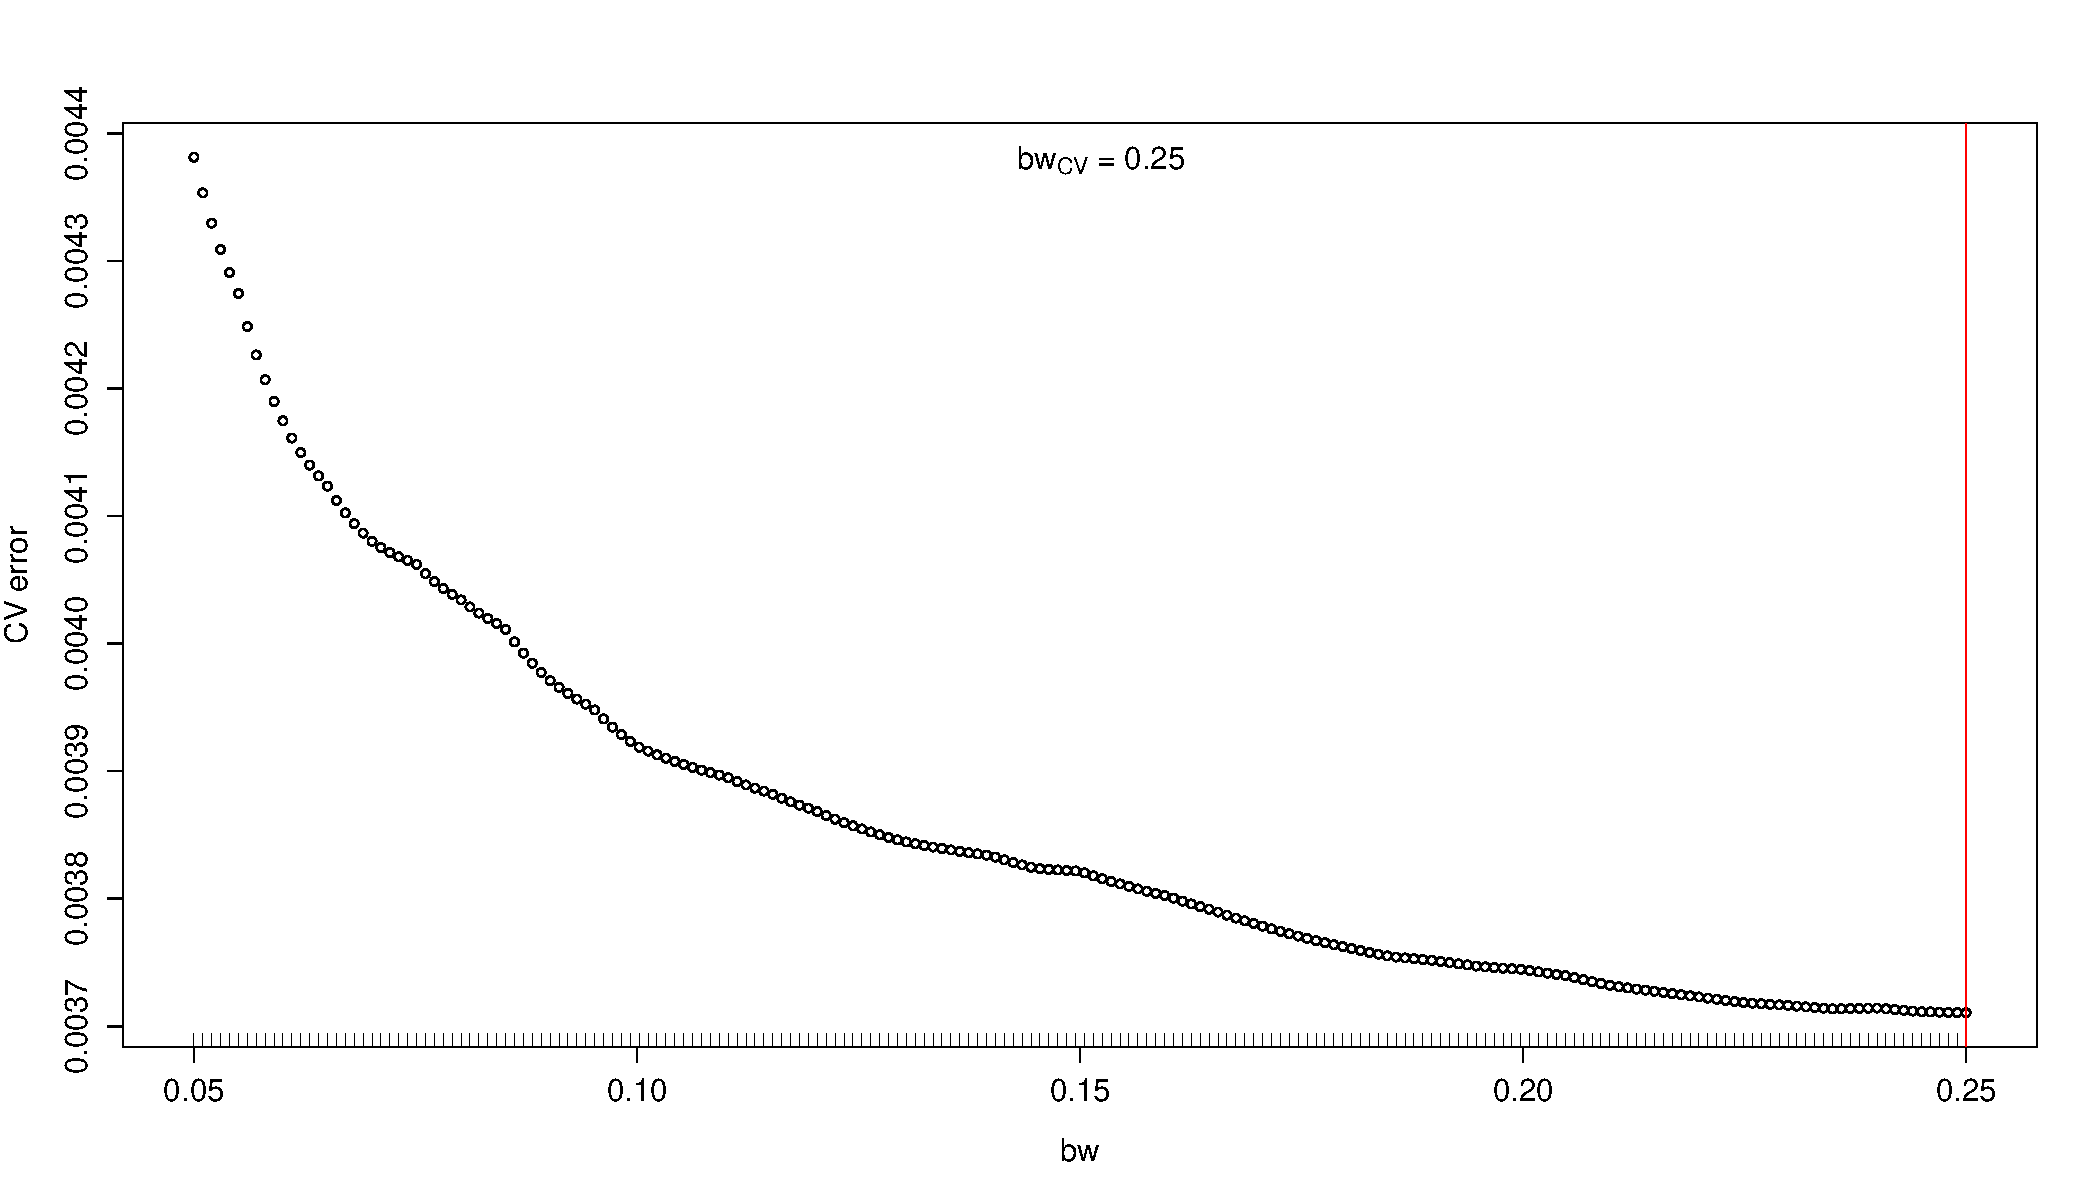
\includegraphics[trim=0 0 20 40, clip, width=\textwidth]{application_figure_03b.pdf}
		\caption{Local linear estimator}
		\label{fig:application_left_ll}
	\end{subfigure}
	\caption{CV error over a grid of 200 bandwidths for the left side to the threshold in Figure~\ref{fig:application_fits}.
			 The optimal bandwidth is indicated by the red line.}
	\label{fig:application_left}
\end{figure}

\begin{figure}
	\centering
	\begin{subfigure}{\textwidth}
		\centering
		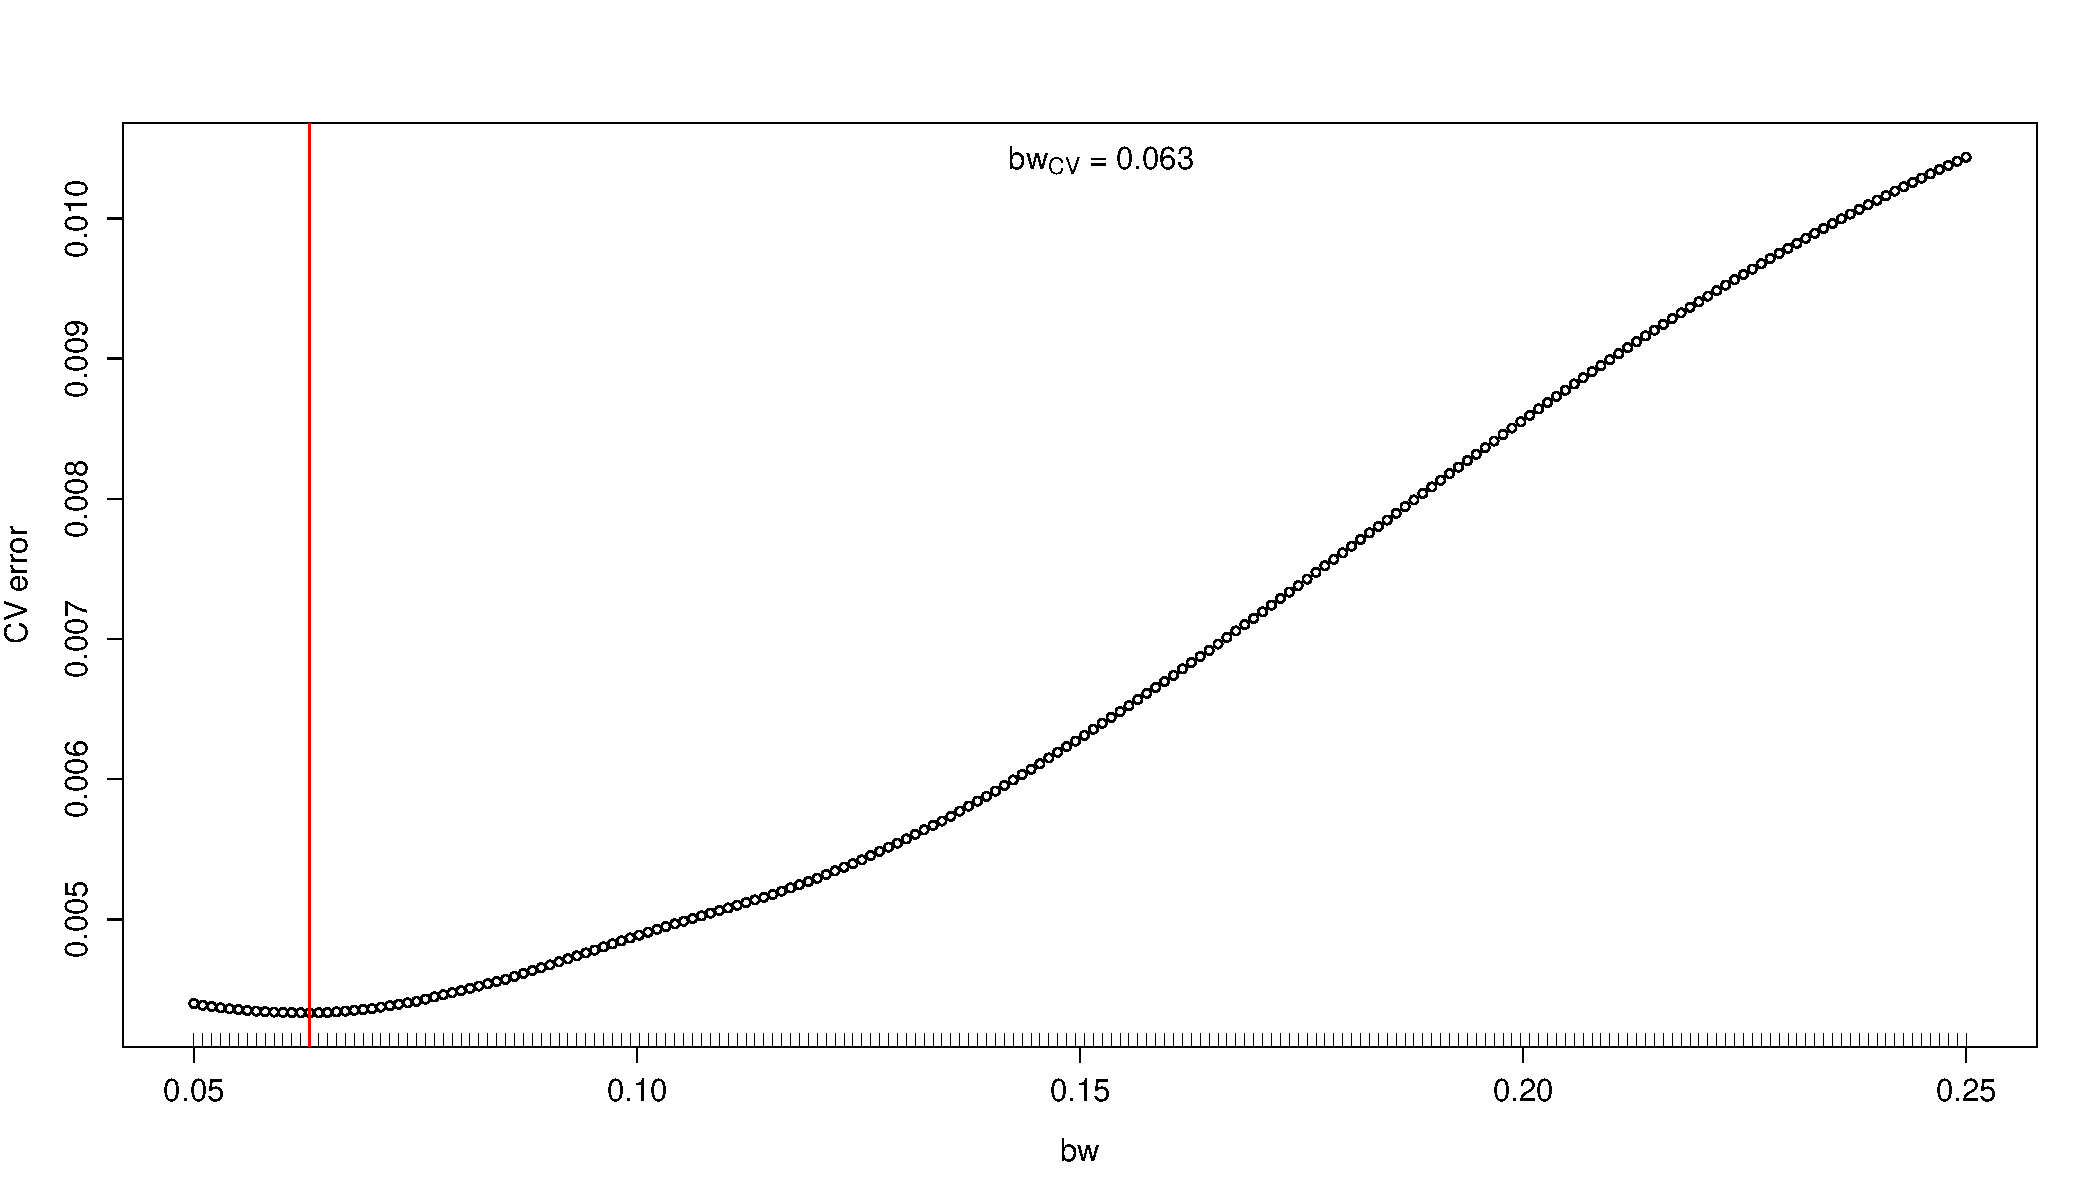
\includegraphics[trim=0 0 20 45, clip, width=\textwidth]{application_figure_04a.pdf}
		\caption{Nadaraya-Watson estimator}
		\label{fig:application_right_nw}
	\end{subfigure}

	\begin{subfigure}{\textwidth}
		\centering
		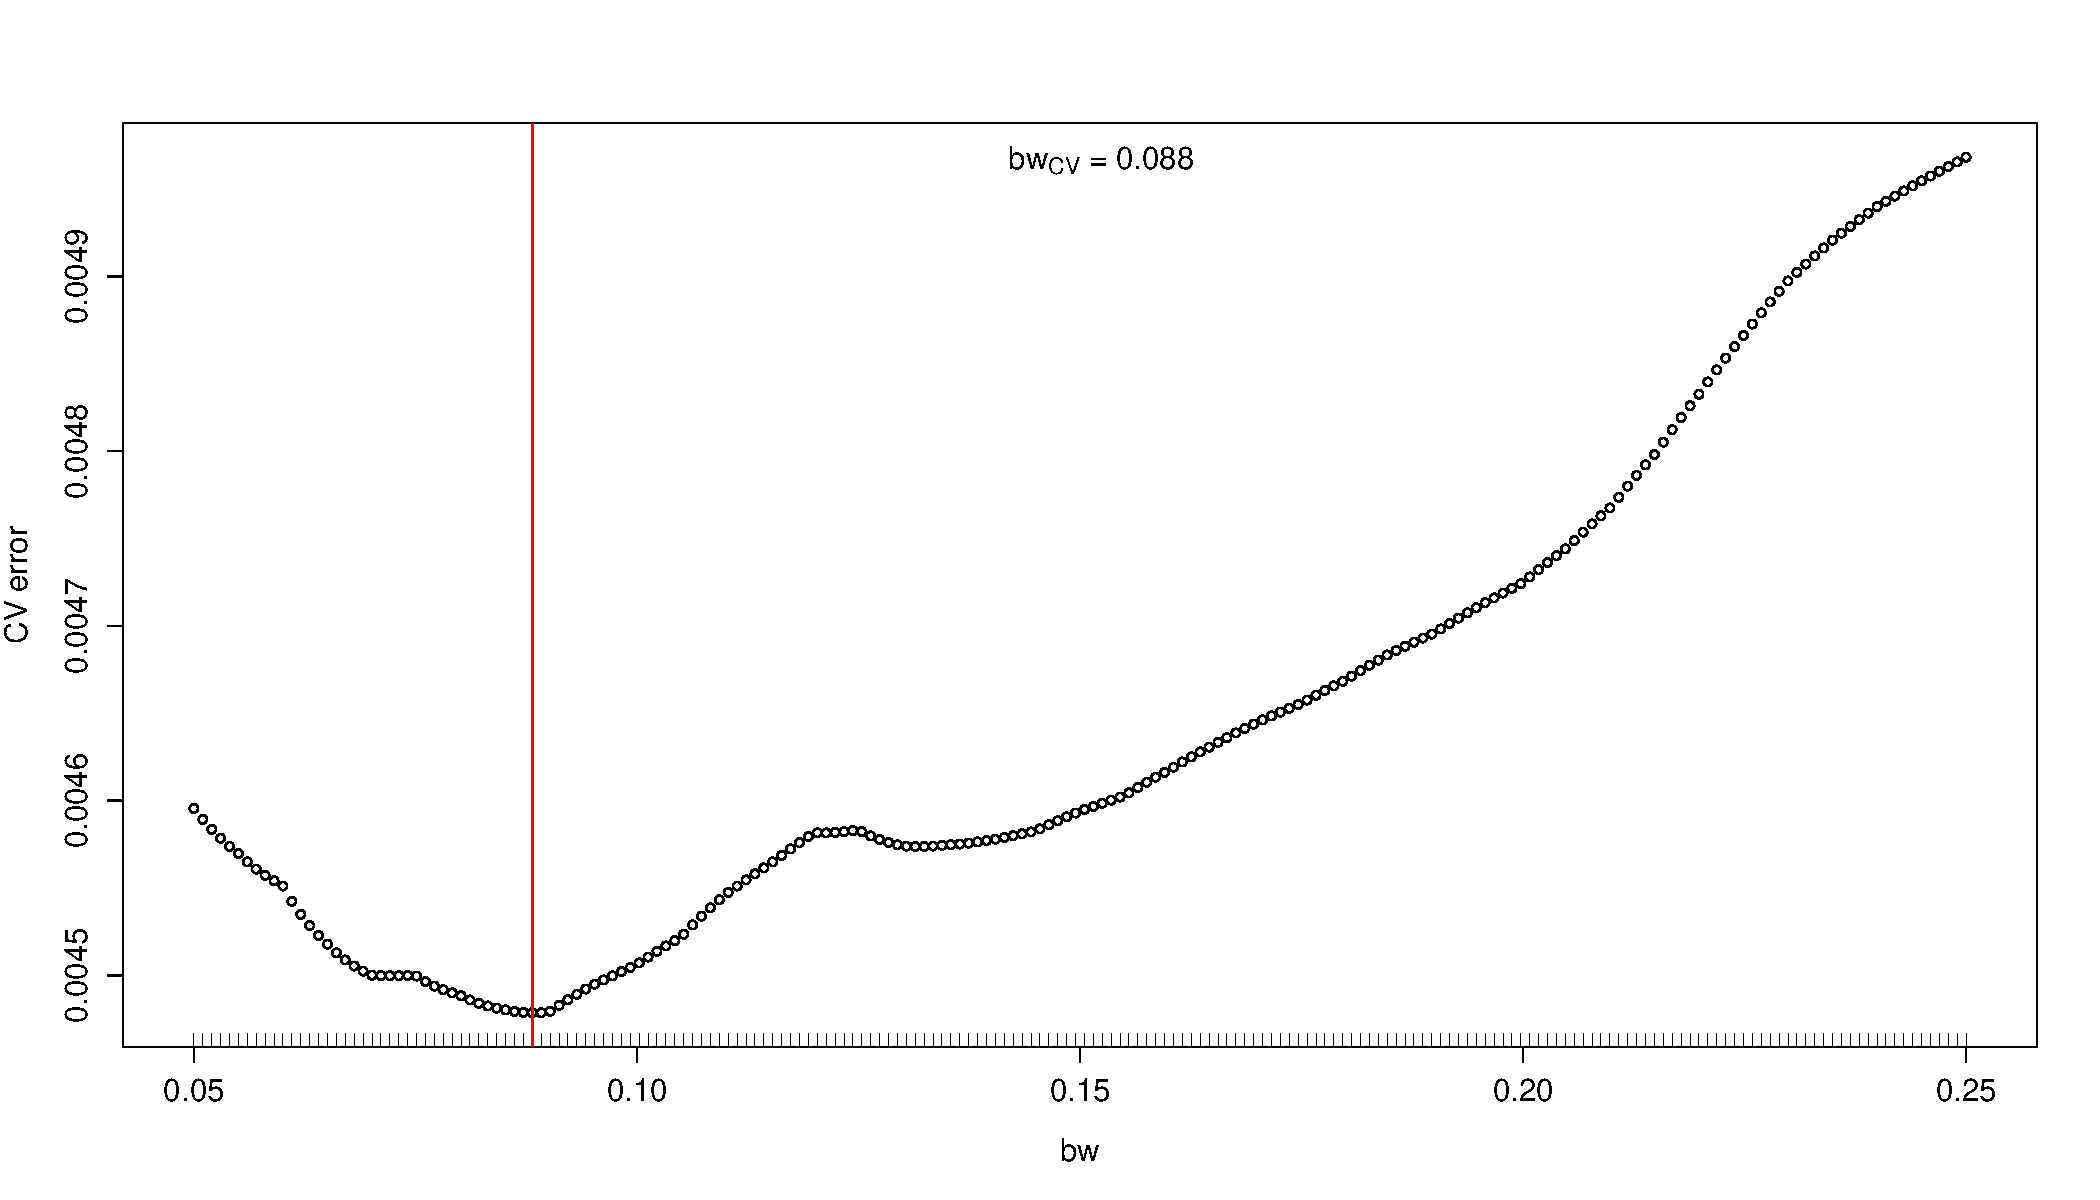
\includegraphics[trim=0 0 20 45, clip, width=\textwidth]{application_figure_04b.pdf}
		\caption{Local linear estimator}
		\label{fig:application_right_ll}
	\end{subfigure}
	\caption{CV error over a grid of 200 bandwidths for the right side to the threshold in Figure~\ref{fig:application_fits}.
			 The optimal bandwidth is indicated by the red line.}
	\label{fig:application_right}
\end{figure}

The estimates to the left side of the threshold look very similar.
However, since local linear regression coincides with the global OLS fit (infinite bandwidth) the estimate is more stable
yet captures the same structure.
In contrast, on the right side the estimates differ considerably near the boundary.
It is apparent that the Nadaraya-Watson estimate suffers from boundary bias.
The explicit boundary adjustment results in a much smaller boundary estimate.
The curve resembles the parametric logit fit of \textcite[Fig.\ 5a]{Lee_2008}.
Local linear regression also leads to a smaller discontinuity estimate, but the correction is less strong.
Besides, the estimate is less wavy.
The figure illustrates the need for boundary correction.
Just looking at the right side to the threshold,
Nadaraya-Watson suggests a ten percentage points greater incumbency advantage compared to adjusted Nadaraya-Watson;
and a more than three percentage points greater advantage compared to the local linear estimator.
Based on Figure~\ref{fig:application_fits} and its simplicity we pick the local linear estimator for further illustration.

We can construct asymptotic confidence intervals to assess precision.
Figure~\ref{fig:application_confidence_bands} displays the local linear estimate along with 95\% approximate confidence bands.
These confidence intervals account for the variance of the estimator but not its bias,
i.e.\ they are not bias-corrected.
We can see that there is more imprecision in the estimator near the threshold.

\begin{figure}
	\centering
	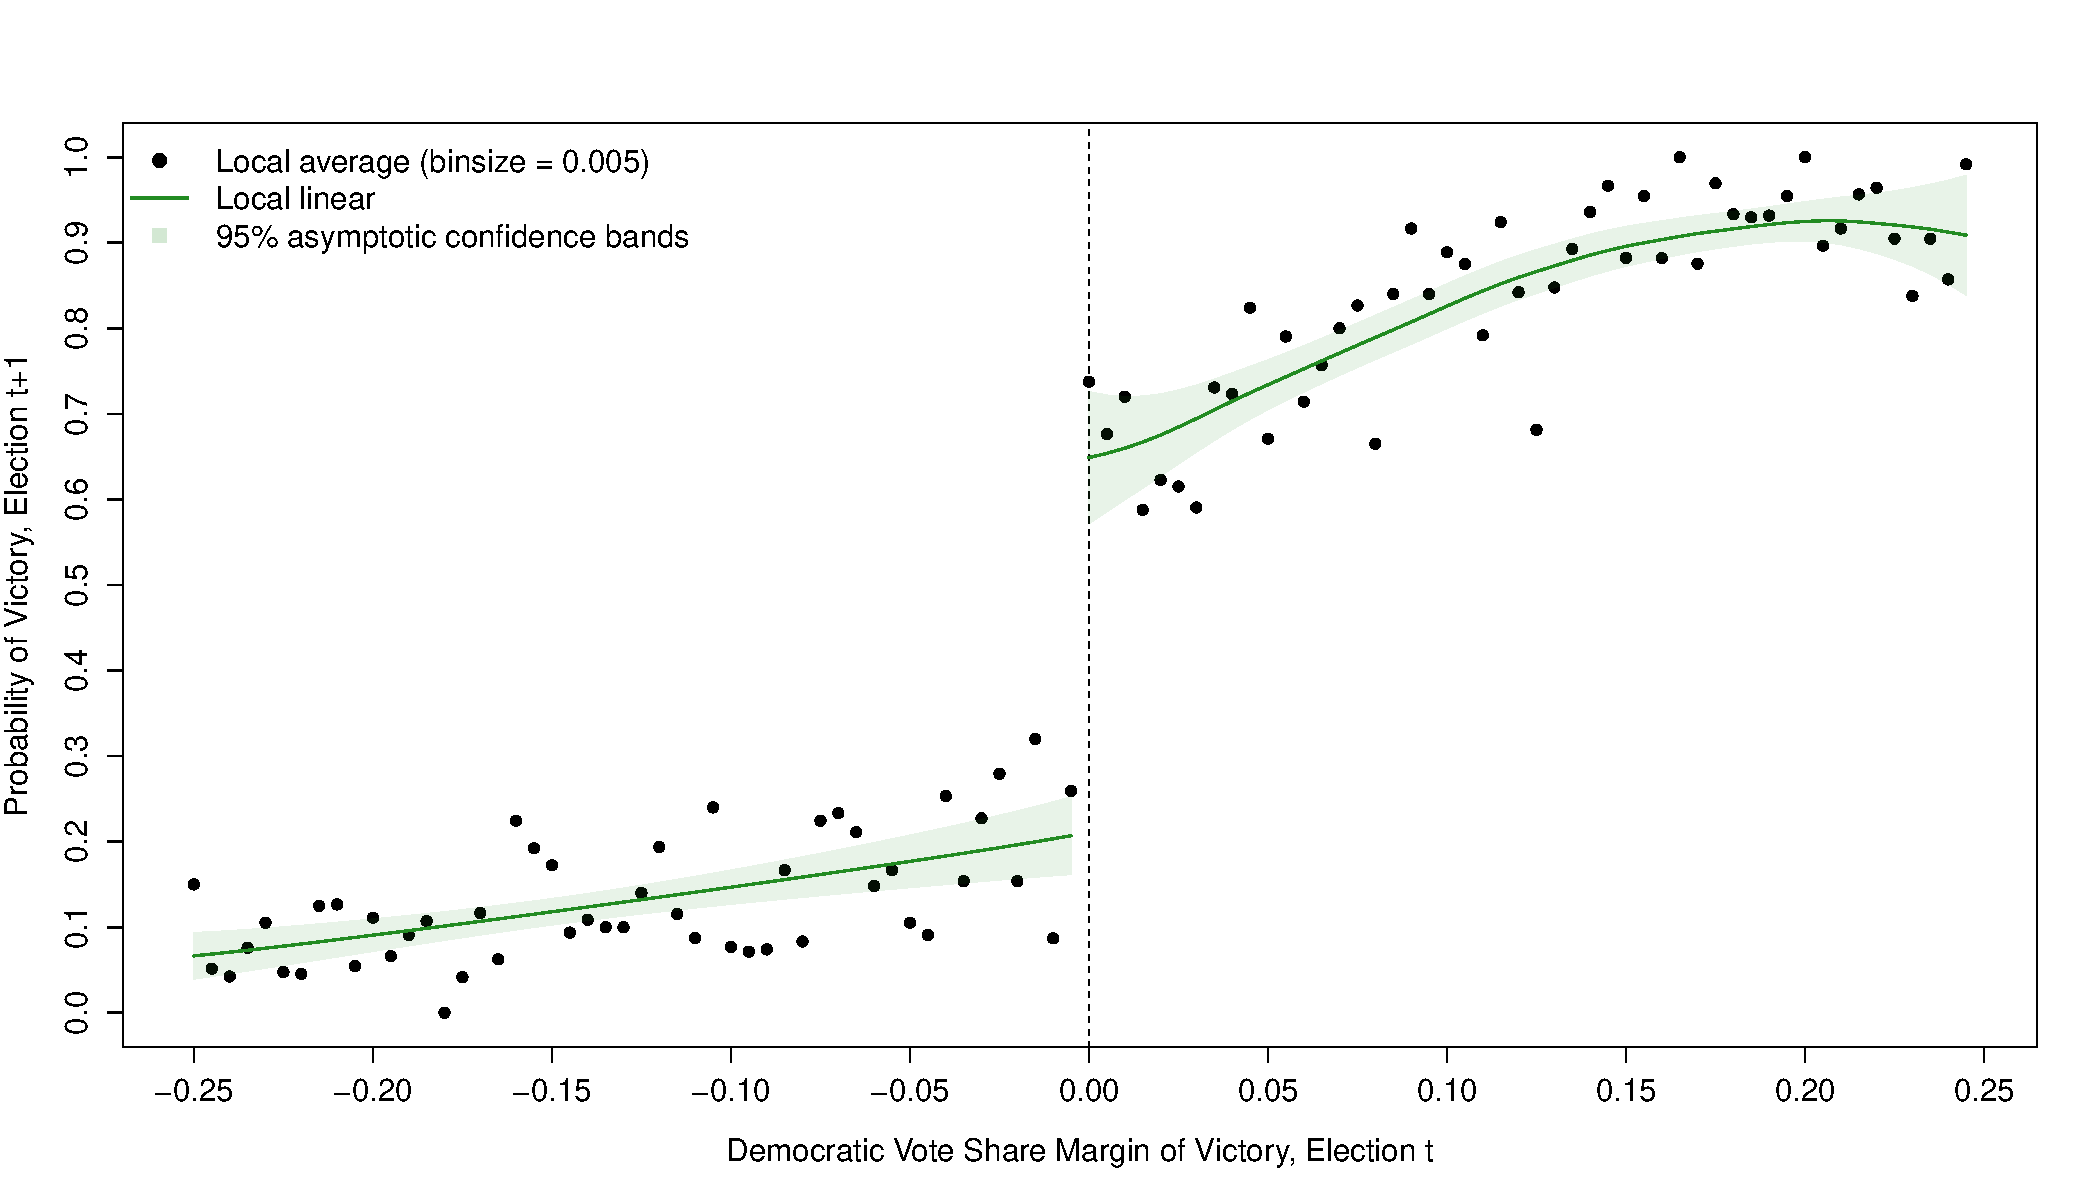
\includegraphics[trim=0 15 20 50, clip, width=\textwidth]{application_figure_05.pdf}
	\caption{Democrats' probability of victory in election $t+1$, by margin of victory in election $t$.
			 Local linear estimate along with 95\% approximate confidence bands.}
	\label{fig:application_confidence_bands}
\end{figure}

\printbibliography

\end{document}